% !TeX root = ../main.tex
% Add the above to each chapter to make compiling the PDF easier in some editors.

\chapter{Method}\label{chapter:method}

A novel method for instance skeletonization of neuronal structures in EM images is proposed. The method is motivated by existing learning based skeletonization method for natural images \cite{Wang2019}, but differs in two distinct ways. First, it separates skeletons for each individual segment - we describe it as instance skeletonization. Second, its is applied on 3D EM images instead of 2D images, which, to the best of our knowledge, has not been explored yet. 
 
\section{Encoding Skeletons in a Vector Field}
Previous skeletonization methods \cite{Shen2016}, \cite{Shen2017}, \cite{Ke2017}, \cite{Wang2019}, \cite{Xu2019} do not separate skeletons of multiple objects. Their prediction is a binary mask marking skeleton points of all salient objects as 'True'. But, in EM images, it is important to separate skeletons of one object instance from another. 
But, it is not straight forward to construct a single Deep Net which can directly demarcate skeletons of object instance. Hence, a encoding must be devised which allows formulating a feasible loss metric and also simple intuitive postprocessing step for decoding skeleton instances. 

\cite{Wang2019} proposes 'Deep Flux' which encodes skeletons of objects in 2D images using a $\mathbb{R}^2$ vector field. It defines a 2D context region around skeleton, and all $\mathbb{R}^2$ vectors in that context region point to the nearest skeleton pixel. This provides a encoding to represent skeletons, and the objective of a Deep Net model would be to predict this field.

The proposed method is also inspired from this encoding, albeit for 3D skeletons and some other tweaks.

Given, ground truth skeletons, a context region is defined for each skeleton, which are the set of points inside a $3D$ ball of $r$ radius.
Let $\Omega \subset \mathbb{Z^3}$  be the 3D image domain consisting of points $\mathbf{p}: (x, y, z)$ and ${\Omega}_s \subset \Omega$ be the set of skeletons points manually labeled. The context set, ${\Omega}_c$ of the skeletons can be defined as

\DeclarePairedDelimiter\norm\lVert\rVert

\begin{equation}
{\Omega}_c := \{ \mathbf{p} \in \Omega \vert \min_{\mathbf{q} \in \Omega_s} \norm{\mathbf{p} - \mathbf{q}}_2 < r \} 
\end{equation}

Further a distance transform $D$ is defined from the skeleton points inside the domain $\Omega$ as

\begin{equation}
\mathbf{D}(\mathbf{p}) := \begin{cases}
		\min_{\mathbf{q} \in \Omega_s} \norm{\mathbf{p}-\mathbf{q}}_2 & \text{if } \mathbf{p} \in \Omega_c \\
		0  & \text{otherwise}
		\end{cases} 
\end{equation}

Finally a $\mathbb{R}^3$ vector field, $\overline{D}$ is obtained by taking discrete gradient of $D$ as follows

\begin{equation}
 \overline{\mathbf{D}}(\mathbf{p}) := \begin{cases}
 \nabla \mathbf{D} & \text{if } \mathbf{p} \in \text{int } \Omega_c \\
 0  & \text{otherwise}
 \end{cases} 
\end{equation}
 
In essence $\overline{\mathbf{D}}$ is a vector field with non-zero direction vectors defined in the vicinity of skeletons, such that the vectors are pointing away from the skeletons, as shown in \autoref{fig:context_field_directions}.

\begin{figure}[htpb]
	\newcommand{\mywidth}{0.45\textwidth}
	\centering
	\begin{subfigure}[b]{\mywidth}
		\centering
		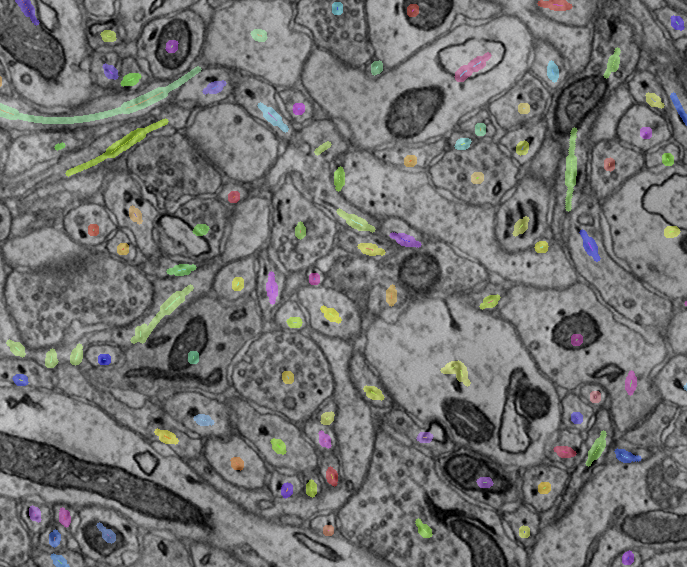
\includegraphics[width=\textwidth]{data/images/contextField/context2D.png}
		\caption{\label{fig:context}}
	\end{subfigure}
	\hspace{3mm}
	\begin{subfigure}[b]{\mywidth}
		\centering
		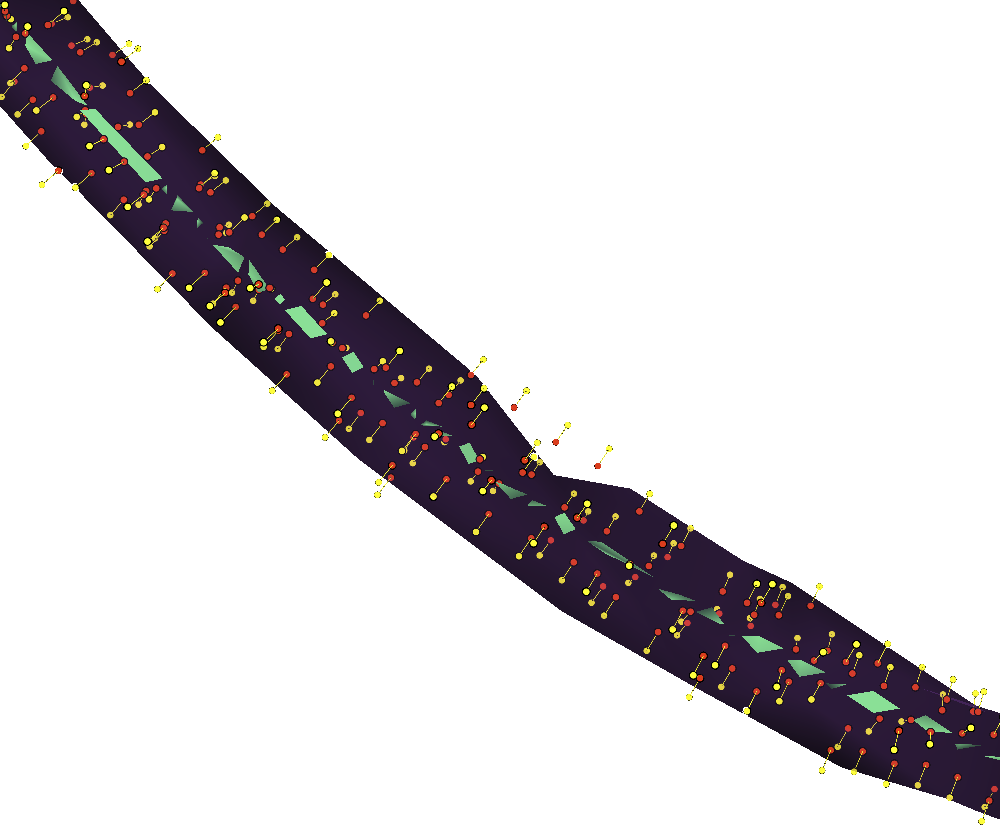
\includegraphics[width=\textwidth]{data/images/contextField/directions_skel_context.png}
		\caption{\label{fig:directions_skel_ctx}}
	\end{subfigure}
		\caption{\subref{fig:context} shows the context for skeletons in a 2D slice. \subref{fig:directions_skel_ctx} shows the field vectors inside the context. They all point away from the skeletons and also follow the shape of the skeleton smoothly}
		\label{fig:context_field_directions}
\end{figure}
	
But, such defined direction field is non-smooth if the skeletons are defined on a discrete grid, shown in \autoref{fig:splineInterpolation}. Learning such a non-smooth field is not encouraged as Deep Nets are usually fail to generate such sharp fields. Hence, to create smoother field, skeleton points are interpolated using splines. Hence, $\Omega_s \subset \mathbb{R}^3$.

\begin{figure}[htpb]
	\newcommand{\mywidth}{0.22\textwidth}
	\centering
	\hspace{3mm}
	\begin{subfigure}[b]{\mywidth}
		\centering
		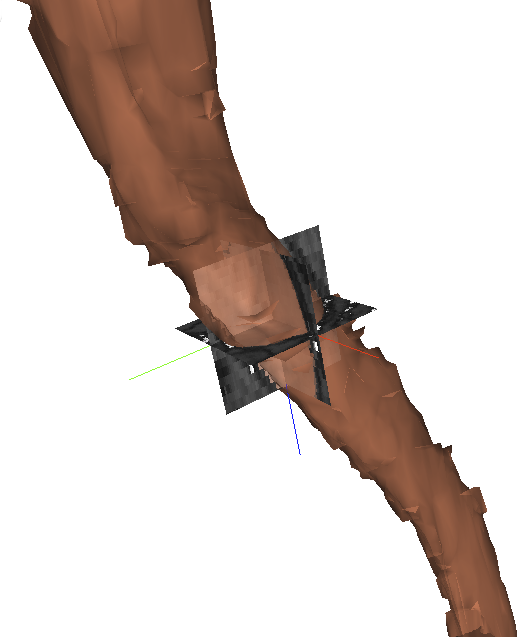
\includegraphics[width=\textwidth]{data/images/interpolation/slice_edited.png}
		\caption{\label{fig:3dseg_slice}}
	\end{subfigure}
	\hspace{3mm}
	\begin{subfigure}[b]{\mywidth}
		\centering
		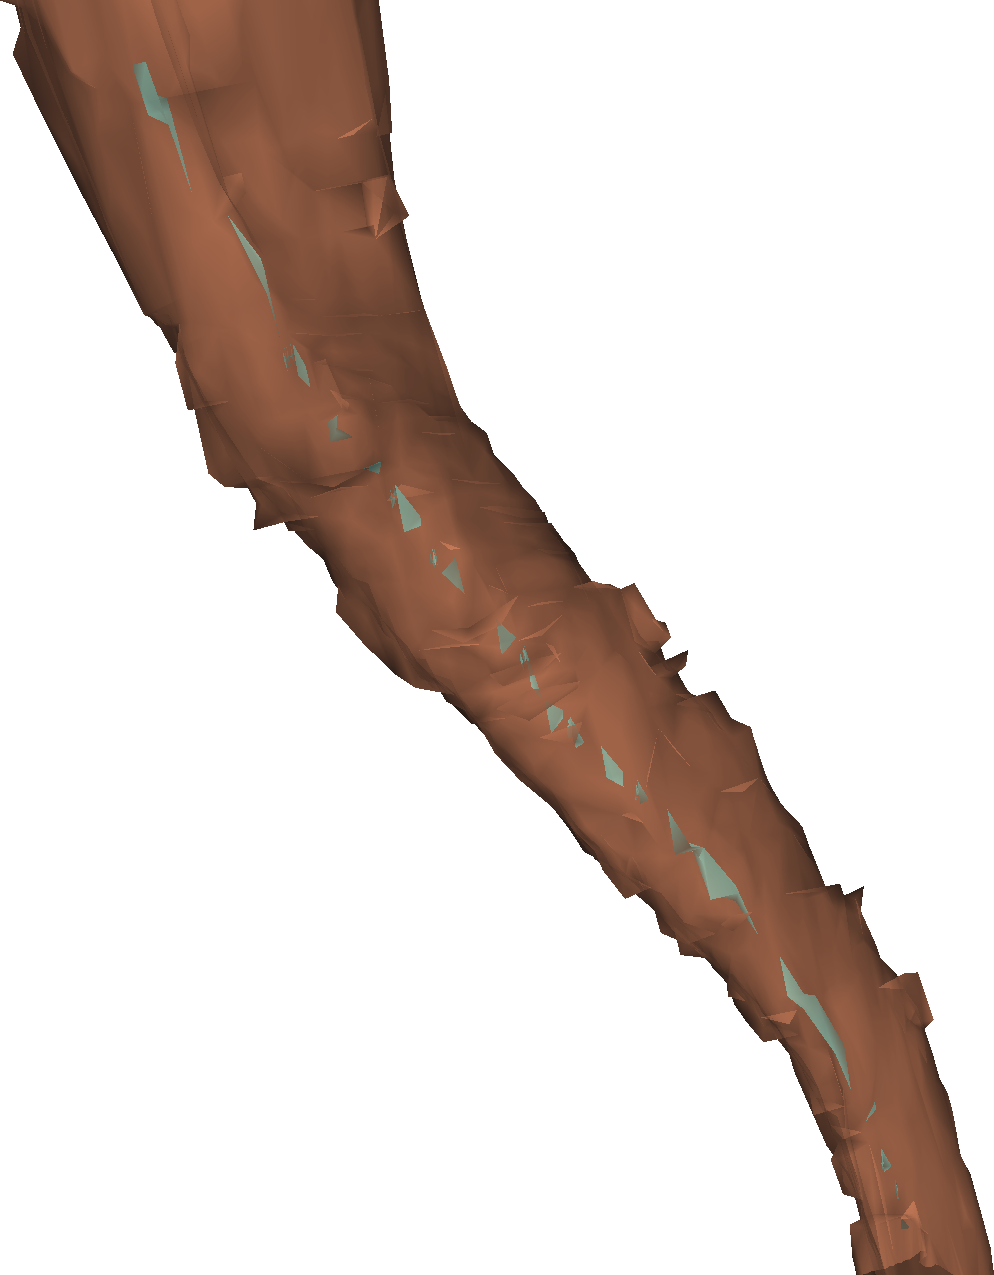
\includegraphics[width=\textwidth]{data/images/interpolation/linear_skel.png}
		\caption{\label{fig:skel_linear}}
	\end{subfigure}
	\hspace{3mm}
	\begin{subfigure}[b]{\mywidth}
		\centering
		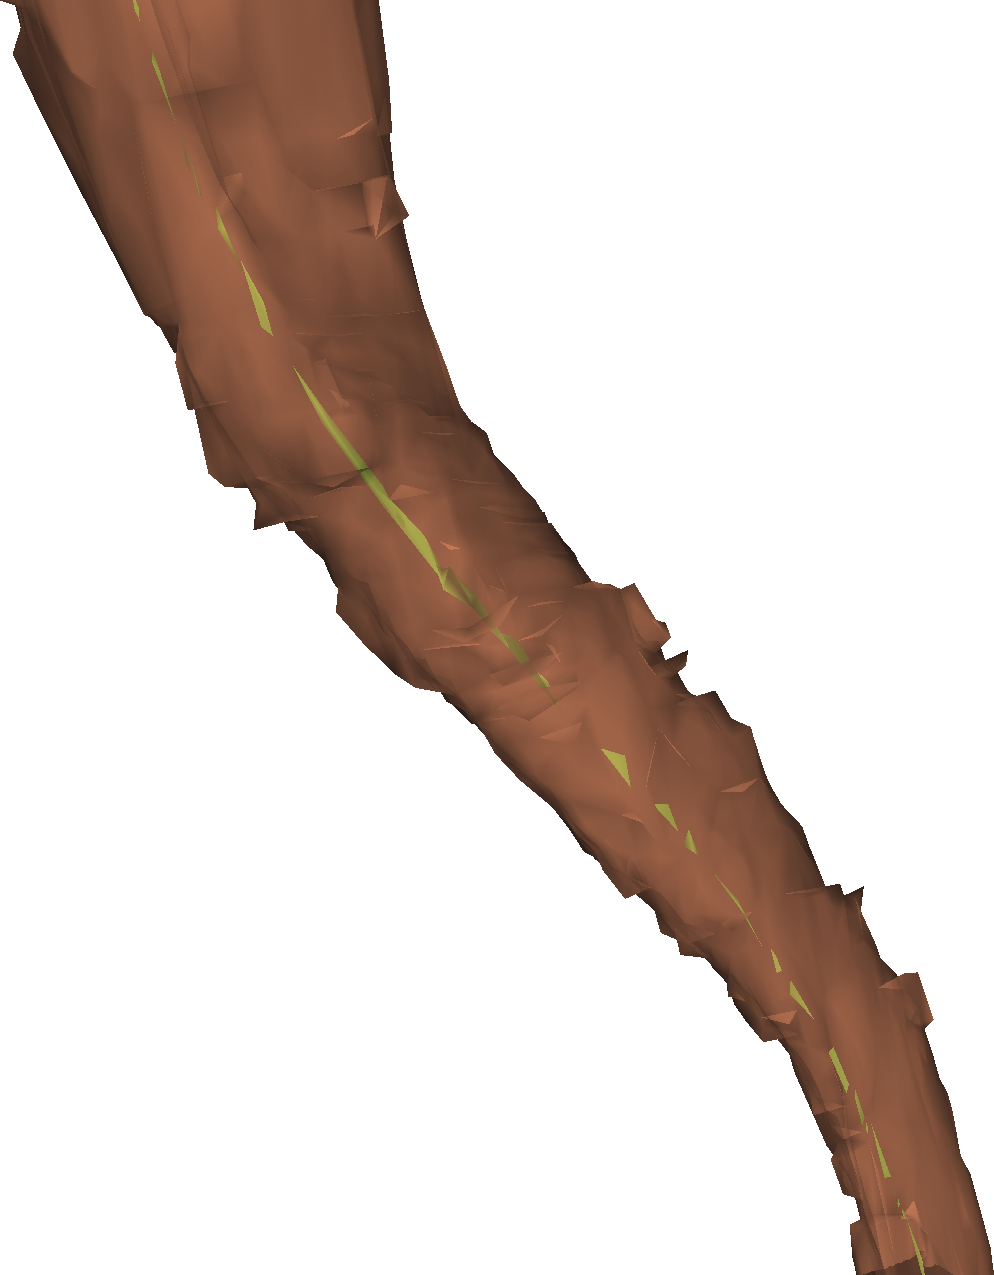
\includegraphics[width=\textwidth]{data/images/interpolation/spline_skel.png}
		\caption{\label{fig:skel_spline}}
	\end{subfigure}\\
	\hspace{3mm}
	\begin{subfigure}[b]{\mywidth}
		\centering
		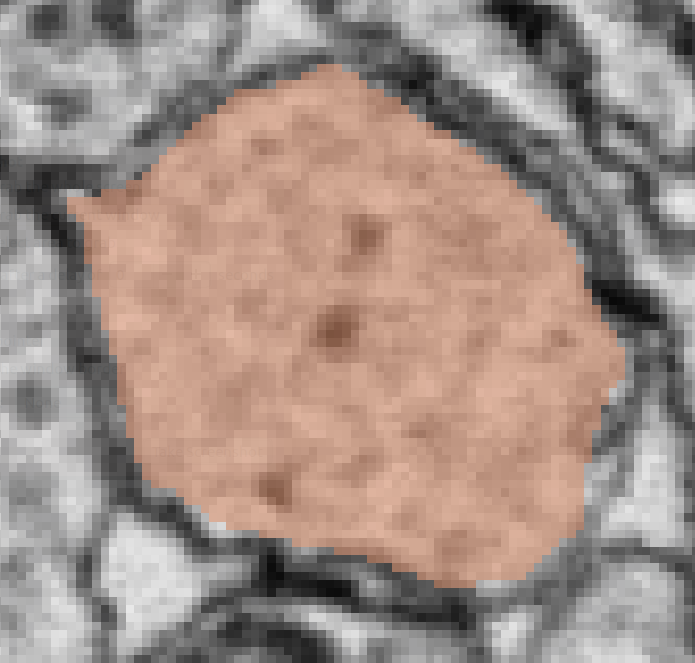
\includegraphics[width=\textwidth]{data/images/interpolation/seg_slice.png}
		\caption{\label{fig:im_seg}}
	\end{subfigure}
	\hspace{3mm}
	\begin{subfigure}[b]{\mywidth}
		\centering
		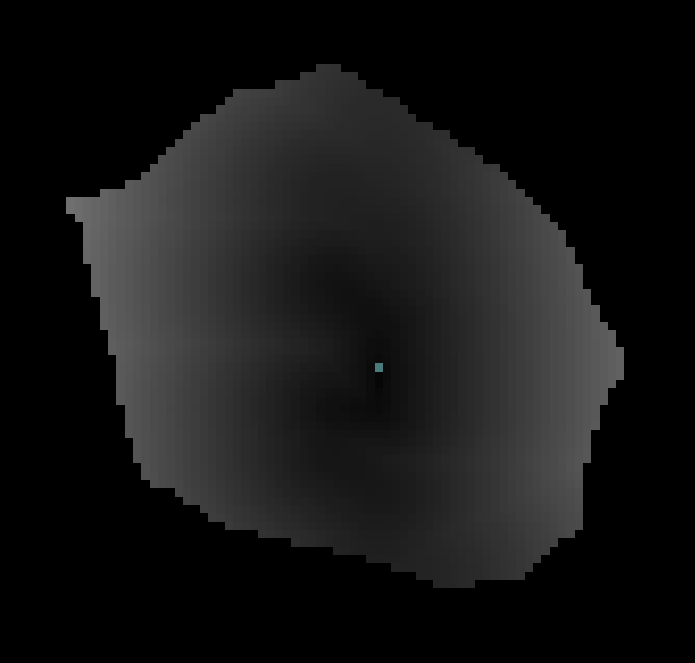
\includegraphics[width=\textwidth]{data/images/interpolation/dtx_linear.png}
		\caption{\label{fig:dtx_linear}}
	\end{subfigure}
	\hspace{3mm}
	\begin{subfigure}[b]{\mywidth}
		\centering
		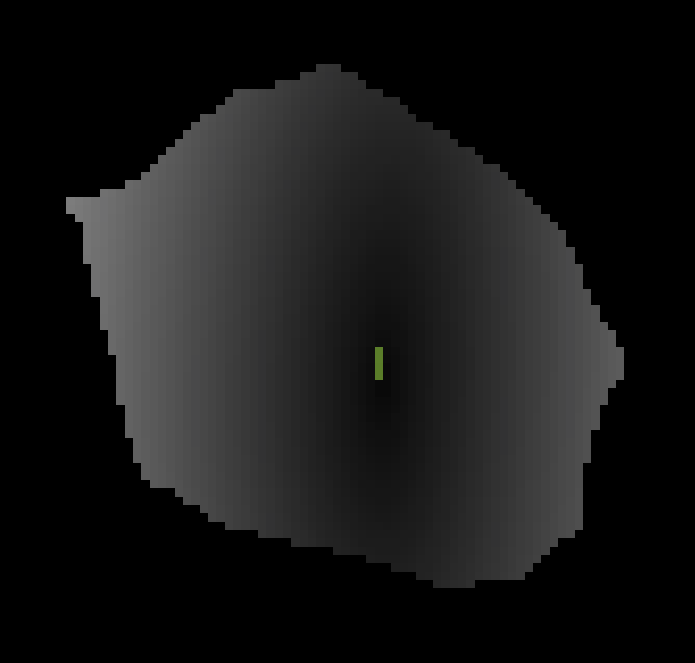
\includegraphics[width=\textwidth]{data/images/interpolation/dtx_spline.png}
		\caption{\label{fig:dtx_spline}}
	\end{subfigure}\\
	\hspace{\mywidth}
	\hspace{3mm}
	\begin{subfigure}[b]{\mywidth}
		\centering
		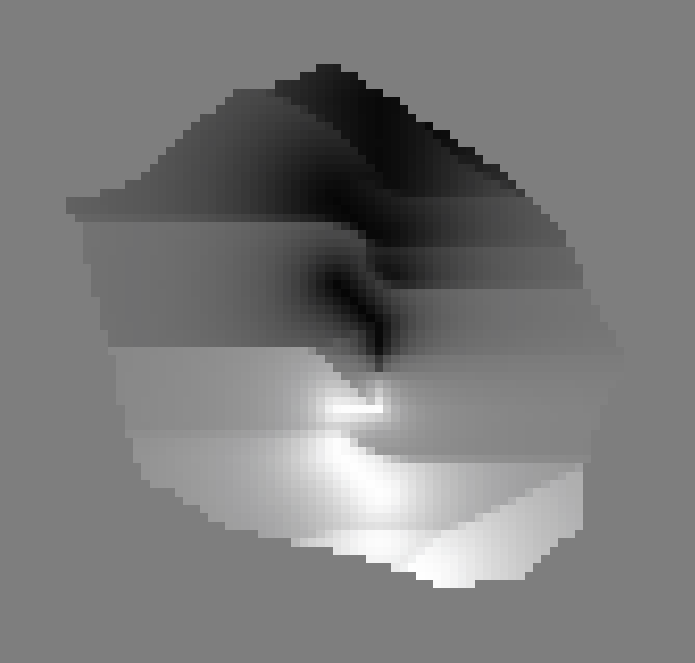
\includegraphics[width=\textwidth]{data/images/interpolation/gradz_linear.png}
		\caption{\label{fig:grad_linear}}
	\end{subfigure}
	\hspace{3mm}
	\begin{subfigure}[b]{\mywidth}
		\centering
		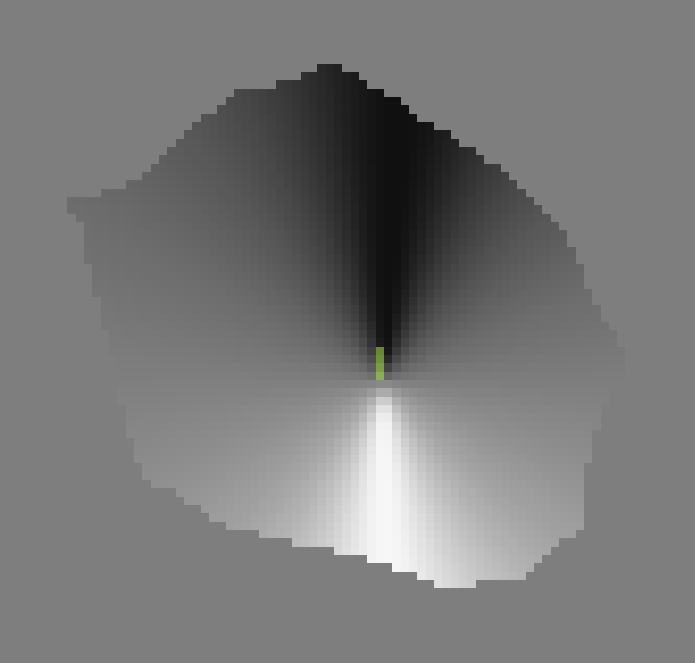
\includegraphics[width=\textwidth]{data/images/interpolation/gradz_spline.png}
		\caption{\label{fig:grad_spline}}
	\end{subfigure}
	\caption{ \subref{fig:skel_linear} and \subref{fig:skel_spline} are resulting skeletons for linearly and spline interpolation methods respectively. \subref{fig:im_seg} is a segment slice in $X-Y$ plane sliced as shown in \subref{fig:3dseg_slice}. \subref{fig:dtx_linear} and \subref{fig:dtx_spline} are the normalized isotropic 3D distance transform from the skeleton for linearly and spline interpolated versions respectively. \subref{fig:grad_linear} and \subref{fig:grad_spline} shows the $z$ component of the gradient of \subref{fig:dtx_linear} and \subref{fig:dtx_spline} respectively. Sharp fields exist in \subref{fig:grad_linear} due to artifacts in the distance transform in \subref{fig:dtx_linear}.}
	\label{fig:splineInterpolation}
\end{figure}


The advantages for encoding skeletons in such a field are:
\begin{itemize}
	\item Deep Net model has to learn to look for both global and local properties while predicting the field. This helps to avoid local false merges due to small membrane breaks, as seen in boundary based methods.
	\item Voxel wise loss function for the deep net can be easily constructed. The loss metric is agnostic of skeleton instances.
	\item Predicted field can be useful to solve false merges and splits in later post processing steps.
\end{itemize}

\section{Network Architecture}
Input to the network is a grayscale image and output is 3 channel vector field.
The backbone of the network is based on Unet \cite{ronneberger2015}. The encoder and decoder of the Unet has four stages, and a center bottleneck layer, with $8, 16, 24, 32, 40$ filters respectively. Each stage of Unet consists of a 3D convolution layer and a residual block. Each residual block made up of two 3D convolution layers with kernel size 3, a short skip connection and ELU nonlinearity. Since EM images have anisotropic resolution, the first and the last stages of the Unet has only 2D convolutions. This is done keeping in mind that first stage can extract information from the high resolution 2D slices and later stages can combine them to extract higher level of information and be resistant to inter-slice artifacts. For downsampling and upsampling in encoder and decoder, 3D Maxpool and linear upsampling is used with a factor of 2, with an exception in the first the last stage where 2D Maxpooling and linear upsampling is used. The network has a theoretical field of view of \textcolor{red}{378*378*32, calculate this again}.  

\section{Training Objective}
Though a L2 or L1 loss between target field $\mathbf{T}$ and predicted field $\mathbf{P}$ can be used, but a more stringent loss would be to enforce correct prediction of the directions of the vectors. This forces a sharper prediction and ensures that the network directly learns directions and hence the shape of the neurons. But since, outside the context region of skeletons the vector field has zero magnitude and thus directions are meaningless. So, a weighted combination (\autoref{loss}) of mean square error(\autoref{mse}) and cosine loss (\autoref{cosineLoss}) is used.

\begin{equation}\label{cosineLoss}
\mathcal{L}_{cos}(\mathbf{P}, \mathbf{T}) := \sum_{\mathbf{q} \in \Omega} \mathbf{W}(\mathbf{q})\left( 1 - \frac{\mathbf{P}(\mathbf{q}).\mathbf{T}(\mathbf{q})}{\max(\norm{\mathbf{P}(\mathbf{q})}_2.\norm{\mathbf{T}(\mathbf{q})}_2,\,\epsilon)} \right)
\end{equation}

\begin{equation} \label{mse}
\mathcal{L}_{mse}(\mathbf{P}, \mathbf{T}) := \sum_{\mathbf{q} \in \Omega} \mathbf{W}(\mathbf{q}) \norm{\mathbf{P}(\mathbf{q}) - \mathbf{T}(\mathbf{q})}_2^2
\end{equation}

\begin{equation} \label{loss}
\mathcal{L} := \alpha\mathcal{L}_{cos} + (1-\alpha)\mathcal{L}_{mse}
\end{equation}

\begin{figure}[htpb]
	\newcommand{\mywidth}{0.3\textwidth}
	\centering
	\begin{subfigure}[b]{\mywidth}
		\centering
		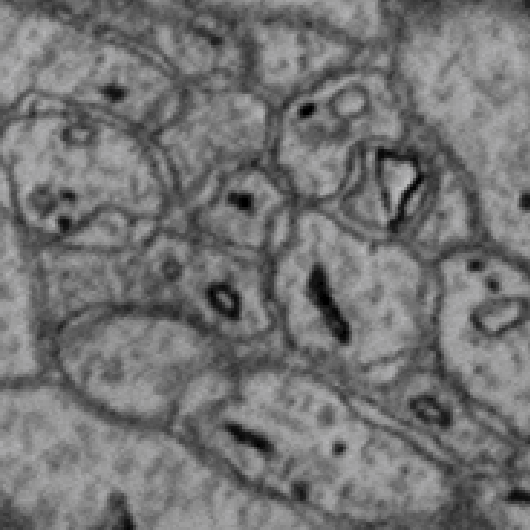
\includegraphics[width=\textwidth]{data/images/fieldLearning/fi_image.png}
		\caption{\label{fig:fi_im}}
	\end{subfigure}
	\hspace{3mm}
	\begin{subfigure}[b]{\mywidth}
		\centering
		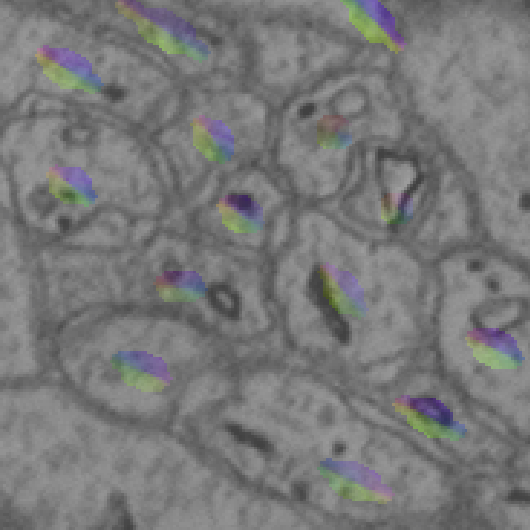
\includegraphics[width=\textwidth]{data/images/fieldLearning/fi_im_field.png}
		\caption{\label{fig:fi_im_f}}
	\end{subfigure}\\
	
	\begin{subfigure}[b]{\mywidth}
		\centering
		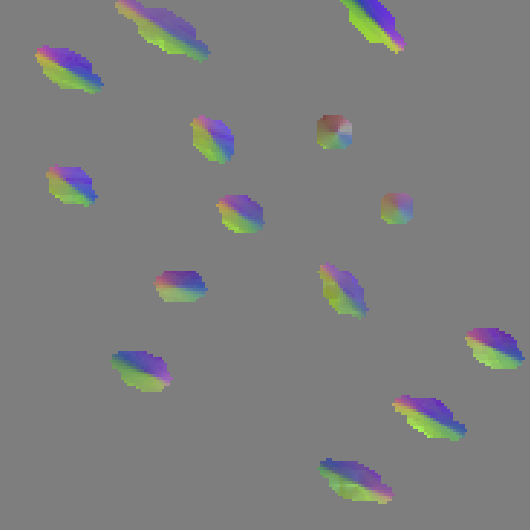
\includegraphics[width=\textwidth]{data/images/fieldLearning/fi_field.png}
		\caption{\label{fig:fi_f}}
	\end{subfigure}
	\hspace{3mm}
	\begin{subfigure}[b]{\mywidth}
		\centering
		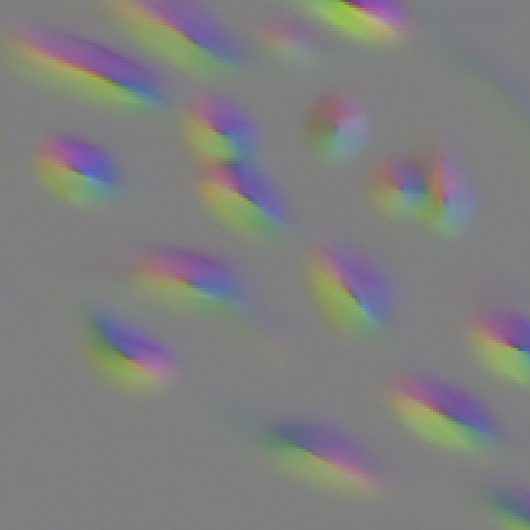
\includegraphics[width=\textwidth]{data/images/fieldLearning/fi_result.png}
		\caption{\label{fig:fi_r}}
	\end{subfigure}
		
	\caption{\subref{fig:fi_im} and \subref{fig:fi_f} shows an 2D slice of input data and the ground truth field. They are overlaid and showed in \subref{fig:fi_im_f}. \subref{fig:fi_r} shows the predicted field.}
	\label{fig:learnedField}
\end{figure}

\section{Decoding Skeletons from Vector Field}
To obtain the instance skeletons back from such an encoding, simple postprocessing steps can be used. First observation about the predicted field is: in the vicinity of skeleton voxels they point away from each other, while at non skeleton voxels they point almost in the same direction. This property can be used to identify skeleton voxels. Divergence at skeleton points would be high, where as for all other location it would be low. And thus thresholding the divergence would allow to create a skeleton mask. Finally, for separating instance skeletons, connected components analysis can be performed.

\section{Splitting and Matching}
After connected component analysis, instance skeletons of most cells can be obtained. But, some skeletons of small and closely located segments are falsely merged, also some skeletons are broken due to irregular shapes and artifacts. To improve such skeletons, another post processing step is devised. 
All false merges occur as junction points of skeletons. So, Junction points are located and the skeletons are split at those locations by a cutting plane along the two eigen vectors with least eigen value.
This results in over-split skeletons, but with almost no false merges.
Finally to merge split skeletons, a classifier is trained to predict if a pair of skeleton requires to be merged. The input to the classifier is a small cropped 3D volume of EM image around the center of the two end points of the skeleton, also combined with it are the cropped skeletons mask in separate channels and the predicted field.

\begin{figure}[htpb]
	\centering
	\begin{subfigure}[b]{0.3\textwidth}
		\centering
		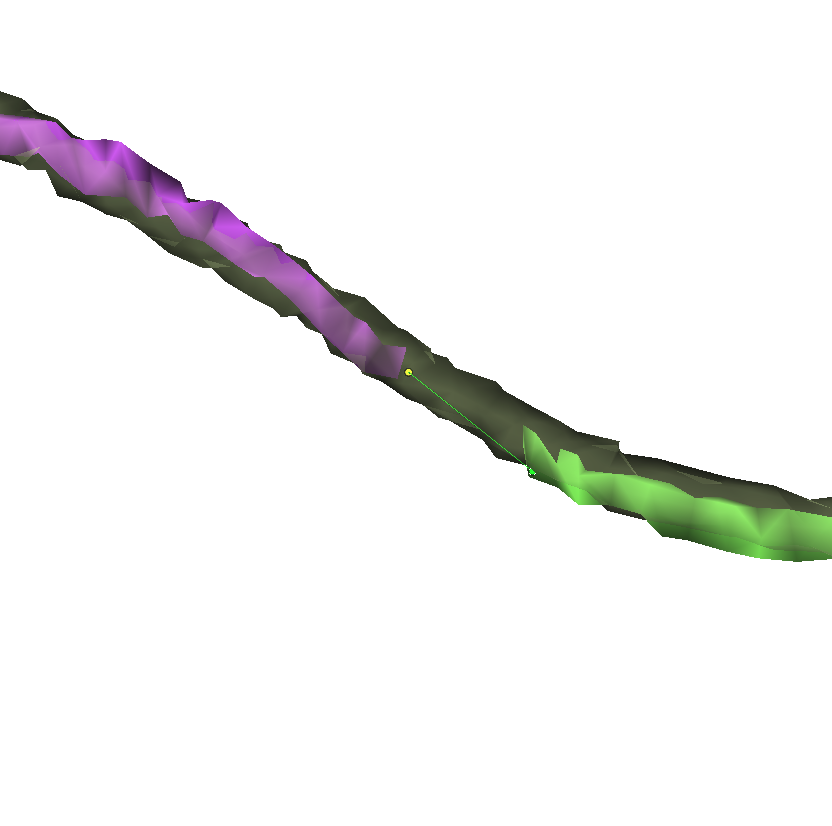
\includegraphics[width=\textwidth]{data/images/matchingData/positive_2.png}
		\caption{\label{fig:positiveMatch}}
	\end{subfigure}
	\hspace{3mm}
	\begin{subfigure}[b]{0.3\textwidth}
		\centering
		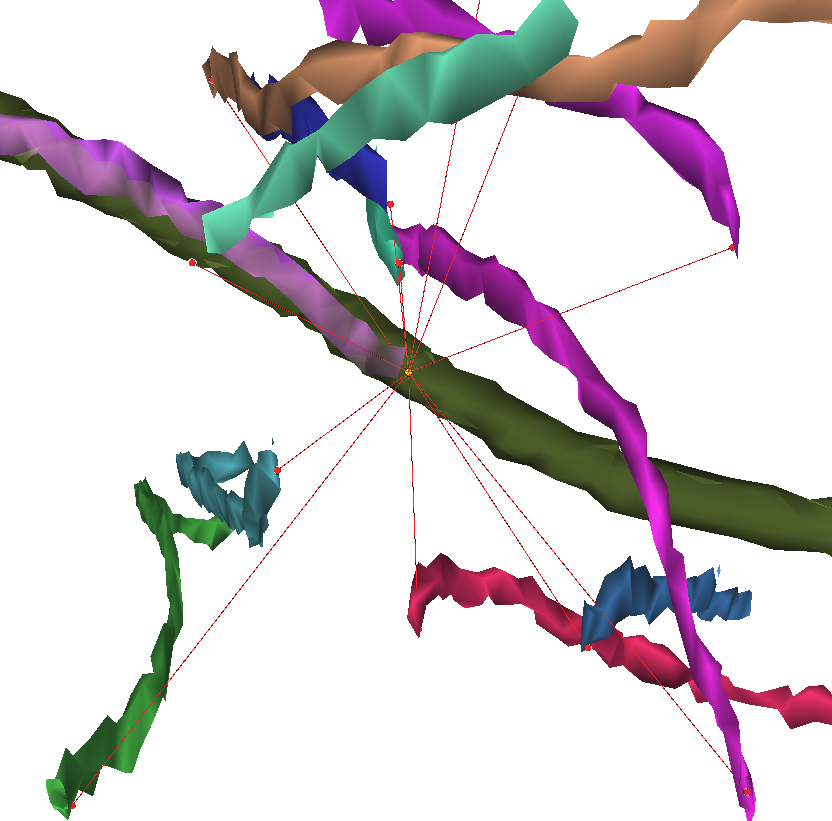
\includegraphics[width=\textwidth]{data/images/matchingData/negative_2.png}
		\caption{\label{fig:negativeMatch}}
	\end{subfigure}
	\caption{Positive \subref{fig:positiveMatch} and negative \subref{fig:negativeMatch} training samples for training a classifier to merge skeletons. Each red line in \subref{fig:negativeMatch} pairs two skeletons which are not part of the same segment. Green line in \subref{fig:positiveMatch} represent the skeleton parts from same segment which needs to be matched}
	\label{fig:skelMatchTrainData}
\end{figure}


\begin{figure}[htpb]
	\centering
	\begin{subfigure}[b]{0.24\textwidth}
		\centering
		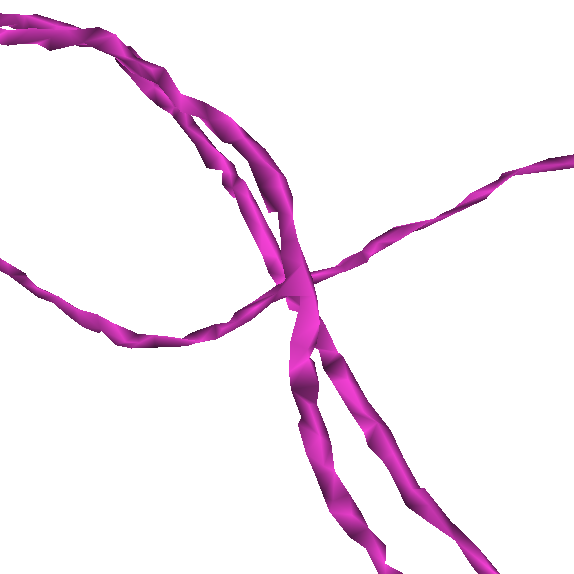
\includegraphics[width=\textwidth]{data/images/splitNMatch/skel.png}
		\caption{\label{fig:splitNMatchA}}
	\end{subfigure}
	\hfill
	\begin{subfigure}[b]{0.24\textwidth}
		\centering
		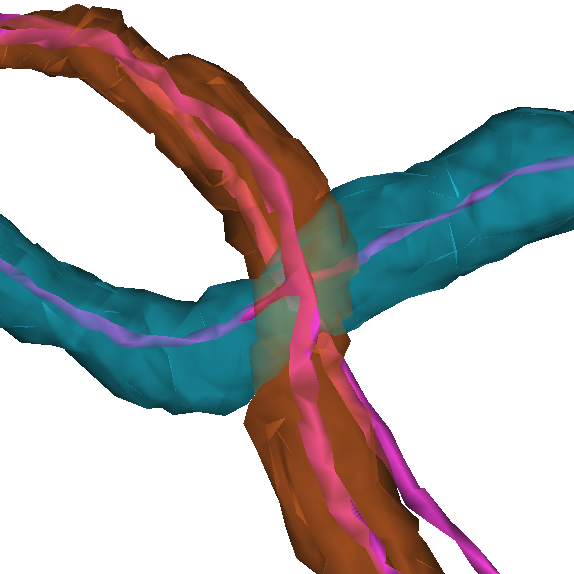
\includegraphics[width=\textwidth]{data/images/splitNMatch/skelNSeg.png}
		\caption{\label{fig:splitNMatchB}}
	\end{subfigure}
	\hfill
	\begin{subfigure}[b]{0.24\textwidth}
		\centering
		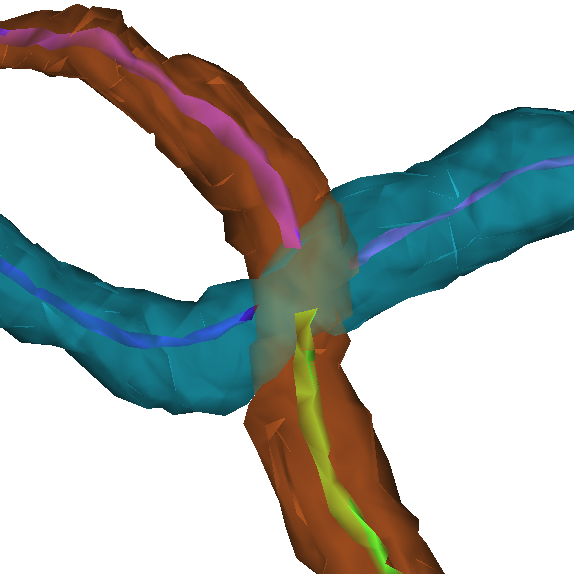
\includegraphics[width=\textwidth]{data/images/splitNMatch/split.png}
		\caption{\label{fig:splitNMatchC}}
	\end{subfigure}
	\hfill
	\begin{subfigure}[b]{0.24\textwidth}
		\centering
		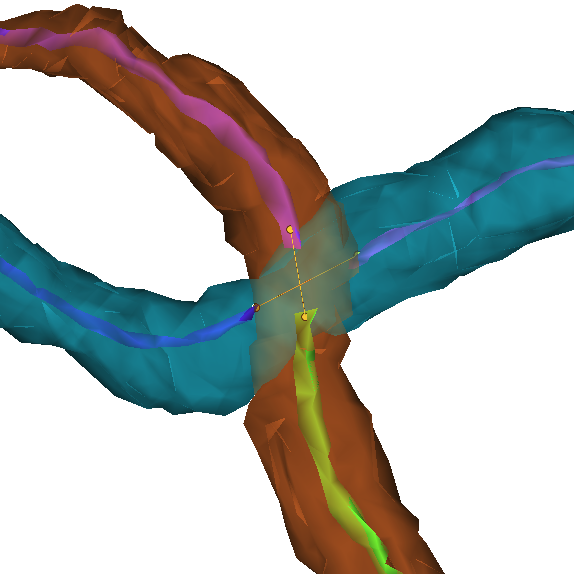
\includegraphics[width=\textwidth]{data/images/splitNMatch/matched.png}
		\caption{\label{fig:splitNMatchD}}
	\end{subfigure}
	\caption{Splitting and matching of skeletons. \subref{fig:splitNMatchA} and \subref{fig:splitNMatchB} shows the falsely merged skeletons. \subref{fig:splitNMatchC} shows skeletons after splitting. Notice that the colors of the skeletons have changed. \subref{fig:splitNMatchD} shows the classifier linking the correct skeletons parts together with yellow lines.}
	\label{skelSplitNMatch}
\end{figure}
